\chapter{Advanced Topics in Propagation Modeling}\labch{research-applications}

After presenting the common ray tracing use cases in \refch{applications}, this chapter focuses on advanced research directions in which ray tracing is combined with machine learning to improve computational efficiency and to investigate the spatial structure of multipath propagation.

\section{Machine-Learning-Assisted Ray Tracing}\labsec{ml-assisted-rt}

As already motivated in \refch{path-tracing}, ray tracing faces combinatorial challenges with exhaustive candidate enumeration: the number of potential paths grows exponentially with the number of objects and interaction order, while most candidates are physically invalid. Beyond the purely geometrical acceleration techniques presented in \refch{efficient-path-tracing}, recent advances in machine learning have opened new possibilities across many research fields, and ray tracing is no exception. A natural question arises: can a neural network predict which candidates are likely to be valid, and thus help the ray tracing engine focus its computational resources on promising paths? To answer this question, this section presents a generative path sampler~\sidecite{Eertmans2026NPJWT,Eertmans2025ICMLCN} that assists path discovery while keeping deterministic geometric validation and electromagnetic-field evaluation unchanged. In short, the learned model replaces the exhaustive candidate-enumeration stage of the ray tracing pipeline, while geometric validation and electromagnetic evaluation remain physics-based, as illustrated in \reffig{research-gps-pipeline}.

\begin{figure*}
  \centering
  \inputtikz{ml-pipeline}
  \caption{Classical versus ML-assisted ray tracing pipelines. The exhaustive candidate enumeration stage is replaced by a generative sampler, while geometric validation and electromagnetic evaluation remain physics-based.}
  \labfig{research-gps-pipeline}
\end{figure*}

\subsection{State-of-the-Art Context and Positioning}

The application of machine learning to radio propagation modeling has accelerated in recent years, motivated by the fundamental trade-off between efficiency and accuracy. Traditional empirical models are computationally fast but often insufficiently accurate for modern wireless systems, while full-wave electromagnetic solvers and high-fidelity ray tracing are precise yet prohibitively expensive at scale. Machine learning offers a compelling middle ground: approximating propagation phenomena with the speed of neural inference. Moreover, the emergence of differentiable programming frameworks has opened new research directions toward end-to-end optimization of wireless systems, spurring interest in differentiable surrogates that can replace or augment conventional simulation tools.

Current machine learning approaches for radio propagation can be organized into several families based on their design philosophy and architectural choices.

\subsubsection{Direct Field and Channel Learning}

Much of the existing literature frames propagation modeling as a supervised learning task, in which neural networks map environmental features directly to channel metrics.

\paragraph{Standard \glsxtrshort{mlp} and \glsxtrshort{cnn}-based approaches} Early methods employed \glspl{mlp} to predict path loss or received power from geometric and environmental features~\sidecite[-8\baselineskip]{Wu2020,Popoola2019,Thrane2020}. For example, \gls{mlp}-based models demonstrated reasonable accuracy in urban and millimeter-wave settings, while \gls{cnn}-based approaches were trained on satellite imagery for path loss prediction at \qty{2.6}{\giga\hertz}. However, these approaches typically require extensive training data and struggle to generalize across different environments or operating conditions, as they are inherently tied to the specific frequencies and material properties of their training distributions.

\paragraph{\Glspl{nerf} and volumetric representations} Inspired by advances in computer graphics, researchers have recently explored using neural radiance fields to represent radio-frequency propagation within complex environments~\sidecite[-7\baselineskip]{Zhao2023,Yang2024,Shen2025}. For instance, \gls{nerf}\textsuperscript{2} introduces a joint training strategy using both synthetic and real-world data to construct a continuous volumetric channel representation. This concept is extended by R-\gls{nerf} to model the dynamic scattering behaviors in \glsxtrshort{ris}-assisted networks. While these approaches can capture complex channel dynamics with impressive precision, they suffer from strict scene-dependence, necessitating a complete, computationally intensive retraining cycle whenever the environment changes. More recently, 3D \gls{gs} models such as \gls{wrf}-\gls{gs} and \gls{rf}-3D\gls{gs} have significantly reduced this overhead, enabling training within minutes and signal queries in milliseconds~\sidecite[-8\baselineskip]{Wen2025,Zhang2026}. Yet, these neural surrogates do not substitute for ray tracing engines; rather, they serve as complementary downstream models that depend on ray-traced datasets for initial training. Consequently, developing faster path sampling techniques directly accelerates the generation of the training data required to bootstrap these representations.

\subsubsection{Alternative and Hybrid Approaches}

Recognizing the challenges of end-to-end field learning, alternative strategies have focused on narrower components of the propagation pipeline or hybrid methods that combine neural networks with physics.

\paragraph{Channel impulse response and trajectory learning} Rather than predicting single metrics like path loss, some models target richer intermediate quantities. To estimate the channel impulse response over spatial regions, physics-informed networks have been developed, capturing both spatial and temporal characteristics~\sidecite{Wang2025}. Other work formulates trajectory generation as a sequential decision problem, treating the synthesis of ray bounces as a sequence-modeling task~\sidecite{Jin2025}. The SANDWICH model, briefly mentioned in \refch{path-tracing}, is a fully differentiable surrogate that learns to generate sequences of bounces, aiming to completely replace the ray tracing simulator.

\paragraph{Neural scene augmentation} An alternative strategy enriches the geometric scene description through neural representations. For instance, neural radiance fields can represent complex objects, allowing standard ray tracing engines to query these representations to account for scattering and diffraction effects that are difficult to model with traditional primitives~\sidecite{Chen2025}.

\subsubsection{Fundamental Limitations of Current Approaches}

Despite these advances, direct field-learning methods face several fundamental challenges that limit their adoption in general-purpose simulation tools.

\paragraph{Highly Oscillatory Field-Mapping Problem}

Models attempting to learn electromagnetic fields directly face a highly sensitive mapping: tiny geometric or frequency perturbations cause significant field fluctuations due to constructive and destructive interference. Learning such highly oscillatory, non-convex spatial functions demands large networks and vast training datasets, often resulting in poor generalization.

\paragraph{Lack of Invariance and Generalization}

Most direct learning models lack invariance to geometric transformations such as rotation or scaling. Furthermore, models are tightly coupled to their training frequencies and material properties. A model trained at \qty{2.4}{\giga\hertz} in an office environment cannot be applied to \qty{28}{\giga\hertz} street canyons without complete retraining. Only recently have researchers explored geometric invariance properties using graph attention architectures~\sidecite{Hehn2024}.

\paragraph{Loss of Physical Interpretability}

End-to-end black-box models discard valuable path-level information. For emerging applications---sensing, localization, and beam management---knowing \emph{which} paths (reflections, diffractions) contribute to the signal is often as important as the final signal strength. This loss of interpretability limits their utility in diagnostic and optimization workflows.

\paragraph{Computational Efficiency Paradox}

While neural inference can be fast, querying large networks may paradoxically be slower than highly optimized geometric ray tracing, especially in simple scenarios. Practical deployment requires that inference overhead be negligible relative to the physics engine it assists.

\subsubsection{Intelligent Path Sampling: A Complementary Approach}

These limitations suggest a different role for machine learning: \emph{guiding} the physics engine rather than replacing it. If neural models learn to \emph{identify} likely valid candidates instead of predicting fields directly, the learning problem becomes less dependent on frequency and material parameters. The model can then focus on geometric regularities, while rigorous field computation remains in the physics solver. This design philosophy motivates the generative path sampler presented next.

\subsection{Methodology}

In this subsection, we show how learning can be integrated into the tracing pipeline while preserving physics-based validation. We proceed through the following components: path construction as sequential sampling, transform-invariant scene encoding, \gls{gflownet}-based policy learning, training-objective optimization, and sparse-reward stabilization.

\subsubsection{From Exhaustive Search to Sequential Sampling}

As discussed in earlier chapters, exhaustive point-to-point tracing is equivalent to exploring all branches of the image tree. For a scene with $N$ candidate objects and interaction order $K$, this exploration scales combinatorially, while only a small fraction of candidates satisfy geometric constraints.

Recent approaches reformulate candidate construction as a sequential decision process. Starting from an empty candidate, one object is appended at each step until a complete length-$K$ sequence is obtained (\reffig{research-gps-path-candidates}). In this framework, a state corresponds to a partial path $\bsit{I}$, and each action selects the next object index to extend that path. The 2D geometry and resulting decision tree in \reffig{research-gps-sequential-geometry} and \reffig{research-gps-sequential-tree} (combined in \reffig{research-gps-sequential}) illustrate how geometric constraints prune infeasible branches. This reformulation converts the exhaustive graph traversal into policy-guided sampling over the same search space.

\begin{figure*}
  \centering
  \inputtikz{path-candidates-tree}
  \caption{Sequential construction of complete path candidates up to interaction order $K$, adapted from the image tree in \reffig{image-tree} with incomplete path candidate notation for intermediate states.}
  \labfig{research-gps-path-candidates}
\end{figure*}

\begin{figure*}
  \centering
  \begin{subfigure}[b]{0.47\contentwidth}
    \inputtikz{path-candidates-sequential-decision-geometry}
    \caption{2D geometry.}
    \labfig{research-gps-sequential-geometry}
  \end{subfigure}
  \hfill
  \begin{subfigure}[b]{0.47\contentwidth}
    \inputtikz{path-candidates-sequential-decision-tree}
    \caption{Decision tree.}
    \labfig{research-gps-sequential-tree}
  \end{subfigure}
  \caption{Simple 2D geometry and resulting decision tree for a path tracing scenario where some interactions can be pruned because an object is unreachable.}
  \labfig{research-gps-sequential}
\end{figure*}

\subsubsection{Transform-Invariant Scene Encoding}

To reduce sensitivity to absolute coordinates, scene geometry is mapped to a canonical \gls{tx}-\gls{rx} frame. With transmitter and receiver positions $\bsup{x}_{\text{\glsxtrshort{tx}}}$ and $\bsup{x}_{\text{\glsxtrshort{rx}}}$, the basis vector aligned with the \gls{line-of-sight} is defined by
\begin{equation}
  \uvec{w} = \frac{\bsup{x}_{\text{\glsxtrshort{rx}}} - \bsup{x}_{\text{\glsxtrshort{tx}}}}{s}
  \quad \text{with} \quad
  s = \|\bsup{x}_{\text{\glsxtrshort{rx}}} - \bsup{x}_{\text{\glsxtrshort{tx}}}\|.
\end{equation}
To preserve a consistent vertical orientation, the remaining orthonormal axes are constructed from the global vertical unit vector $\uvec{e}_z=[0,0,1]^\top$ as
\begin{equation}
  \uvec{u}=\frac{\uvec{w}\times\uvec{e}_z}{\|\uvec{w}\times\uvec{e}_z\|},
  \qquad
  \uvec{v}=\uvec{w}\times\uvec{u}.
\end{equation}

When $|\uvec{w}\cdot\uvec{e}_z|\approx 1$ (near-vertical \gls{tx}--\gls{rx} alignment), this construction becomes singular because $\uvec{w}\times\uvec{e}_z\approx\bsup{0}$. In that case, a fallback reference axis (e.g., $\uvec{e}_x$) is used to build the orthonormal basis and avoid division by zero.

With the rotation matrix $\bsit{R}=[\uvec{u},\uvec{v},\uvec{w}]^\top$, each scene vertex $\bsup{x}_i$ is transformed as
\begin{equation}
  \bsup{x}'_i = \bsit{R}\left(\frac{\bsup{x}_i-\bsup{x}_{\text{\glsxtrshort{tx}}}}{s}\right),
\end{equation}
so that the transmitter maps to $
\begin{bmatrix}0 & 0 & 0
\end{bmatrix}^\top$ and the receiver to $
\begin{bmatrix}0 & 0 & 1
\end{bmatrix}^\top$. This normalization improves transfer across scenes by factoring out global translation, scale, and azimuthal orientation.

\subsubsection{\glsxtrshort{gflownet}-Based Path Sampling}

\begin{figure*}
  \centering
  \inputtikz{ml-model}
  \caption{Neural architecture of the generative path sampler (object/state/scene encoders + flow head).}
  \labfig{research-gps-model}
\end{figure*}

The neural architecture (detailed in \reffig{research-gps-model}) consists of three main components: an object encoder, a state encoder, and a flow head. The object encoder processes the geometric features of each scene primitive (transformed to the canonical frame), which in this case consist only of the object's vertex coordinates. Because the set of candidate objects is inherently unordered, a \emph{Deep Sets} architecture~\sidecite{Zaheer2017} is used to encode the objects into a single scene embedding. This choice is motivated by the need for permutation invariance, ensuring that the model's predictions do not depend on the arbitrary indexing of objects in the scene. Compared to attention-based architectures such as Transformers, Deep Sets offer superior scalability---linear $\mathcal{O}(N)$ complexity versus quadratic $\mathcal{O}(N^2)$---and avoid the need for artificial positional encodings, which is particularly beneficial when handling thousands of objects. Through training, the \glspl{mlp} within these encoders learn high-level spatial embeddings that capture the relative importance of objects for potential interactions based on their geometry and distance from the \gls{tx}--\gls{rx} axis.

Sampling is modeled with a \gls{gflownet} over partial candidates. The goal is to learn a forward probability distribution (called the \emph{policy}) $\pi(\bsit{I}'\mid\bsit{I})$ such that complete valid paths are sampled with probability mass proportional to a reward function expressed as
\begin{equation}
  P(\bsit{I}) \propto R(\bsit{I}),
\end{equation}
for terminal states $\bsit{I}$. In this context, a binary reward captures path validity and is defined as
\begin{wideequation}
  R(\bsit{I}) =
  \begin{cases}
    1, & \text{if }\text{path tracing}(\text{\glsxtrshort{tx}},\bsit{I},\text{\glsxtrshort{rx}})\text{ is geometrically valid},\\
    0, & \text{otherwise}.
  \end{cases}
\end{wideequation}

Although the reference study uses a strictly binary reward, it may be possible to use a continuous reward. For example, the smoothing mechanism described in \refsec{drt-discontinuities} could be applied to provide more informative feedback for near-valid candidates, thereby improving training dynamics.

Training enforces flow conservation on visited states through the constraint
\begin{equation}
  F(\mathrm{parent}(\bsit{I})\rightarrow\bsit{I}) = R(\bsit{I}) + \sum_{\bsit{I}'\in\mathcal{C}(\bsit{I})}F(\bsit{I}\rightarrow\bsit{I}'),
\end{equation}
where $\mathcal{C}(\bsit{I})$ denotes the children of state $\bsit{I}$. The induced policy is then expressed as normalized outgoing flow values
\begin{equation}
  \pi(o_i\mid\bsit{I}) = \frac{F\left(\bsit{I}\rightarrow\mathcal{T}(\bsit{I},o_i)\right)}{\sum_j F\left(\bsit{I}\rightarrow\mathcal{T}(\bsit{I},o_j)\right)},
\end{equation}
where $\mathcal{T}(\bsit{I},o_i)$ denotes the child state reached by appending object $o_i$ to state $\bsit{I}$.

This mechanism pushes probability mass toward branches that lead to valid complete paths while preserving stochastic exploration. After successful training, the architecture in \reffig{research-gps-model} will only sample geometrically valid candidates. This effect is visible in \reffig{research-gps-sequential}, where the policy suppresses invalid branches and concentrates computation on promising ones.

\subsubsection{Training Objective and Optimization}

In practice, the flow-conservation constraint is optimized through a mean-squared flow-matching loss accumulated over sampled trajectories. At each training iteration, scenes are drawn from a scenario generator (or replay memory), transformed into the canonical frame, and used to sequentially sample one or more candidates up to order $K$. The object encoder, scene encoder, path-state encoder, and flow head are trained jointly via gradient descent.

Because rewards are sparse at higher orders, convergence quality depends strongly on exploration and replay design. The training loop in \reffig{research-gps-training} therefore combines policy-based sampling, replay sampling, and geometric validation feedback. In this context, the model is trained on a \emph{class of scenes}, which we define as a collection of environments sharing similar geometric and topological statistics. For instance, the urban street-canyon class represents outdoor environments with parallel building rows of varying heights and widths, whereas an indoor-office class would consist of interconnected rooms and corridors. By learning on randomized instances within a class, the model generalizes to unseen snapshots of the same environment type, rather than memorizing a single fixed map.

\subsubsection{Training Stabilization Mechanisms}

Because valid paths are exceptionally sparse at high interaction orders, stable learning necessitates careful algorithmic design. To this end, five complementary mechanisms have been investigated:

\begin{itemize}
  \item The \emph{successful-experience replay buffer} allows previously successful scene-path pairs to be revisited during training, mitigating collapse toward trivial low-flow policies.
  \item The \emph{uniform exploratory policy ($\epsilon$-greedy)} samples actions from a uniform distribution $\mathcal{U}$ with probability $\epsilon$ rather than from the learned policy, maintaining discovery of unseen valid branches.
  \item The \emph{physics-based action masking} removes geometrically impossible next interactions from the policy support by leveraging physical constraints (see \refsec{masking-unreachable-objects}).
  \item The \emph{distance-based weighting} reweights outgoing flows using distance priors to bias selection toward geometrically plausible next interactions, though empirical gains are scenario-dependent.
  \item Finally, the \emph{transmitter--receiver symmetry replay} injects reciprocal path pairs during training to encourage symmetry-aware sampling, although reported improvements are not systematic across all settings.
\end{itemize}

The overall training procedure is detailed in \reffig{research-gps-training}, while the action masking and distance-based weighting mechanisms are illustrated in \reffig{research-gps-action-pruning}.

\begin{figure*}
  \centering
  \inputtikz{training-procedure}
  \caption{Training loop with replay sampling, exploratory policy, and path validation feedback.}
  \labfig{research-gps-training}
\end{figure*}

\begin{figure*}
  \centering
  \inputtikz{action-pruning}
  \caption{Action masking used to prune physically invalid transitions during sampling.}
  \labfig{research-gps-action-pruning}
\end{figure*}

These stabilization mechanisms collectively address sparse rewards and enable the network to discover long-range valid paths even at high interaction orders.

\subsection{Study Summary and Main Results}

The presented framework has been evaluated on the Sionna~RT urban street-canyon scenario presented in \refch{applications} (illustrated in \reffig{street-canyon}), with randomized scene variations and interactions up to third order. Its training relied on dynamic scene generation to promote learning of geometric regularities rather than memorization of fixed coordinates.

\subsubsection{Performance Metrics}

Two complementary metrics are used to evaluate the performance of the generative path sampler for a given \emph{sampling budget} $M$ (the maximum number of path candidates generated by the model per receiver):
\begin{itemize}
  \item The \emph{accuracy} is defined as the ratio of valid sampled candidates to total sampled candidates (up to $M$), quantifying the precision of the sampler.
  \item The \emph{hit rate} is the ratio of unique valid paths discovered by the sampler (within the $M$ candidates) to the full set of valid paths (estimated via exhaustive tracing), measuring coverage of the valid-path set.
\end{itemize}

These metrics capture different behaviors: high accuracy can be achieved by repeatedly sampling a small subset of valid paths, whereas a high hit rate requires path diversity and broader exploration.

\subsubsection{Ablation Results}

\reftab{ablation_results} summarizes the main findings reported in the reference study~\sidecite{Eertmans2026NPJWT}. The replay buffer is the dominant component for stability: without replay, third-order training frequently collapses (zero accuracy and hit rate in several settings), whereas replay-enabled configurations reach substantially better third-order performance. Exploratory sampling ($\epsilon$-greedy) further improves coverage, with the best third-order hit rate obtained for the combined replay and exploration setting (\qty{67.5}{\percent}).

Action masking provides moderate gains, especially at higher orders, while distance-based weighting is generally detrimental in the tested setup, often degrading both accuracy and hit rate. Enforcing explicit \gls{tx}-\gls{rx} symmetry does not yield systematic improvements and can hurt third-order performance. For training-scenario ablations, models trained on canyon-focused (referred to as \gls{co}) data with \gls{og} achieve the strongest overall performance, reaching a \qty{97.3}{\percent} hit rate at $K=1$, \qty{92.8}{\percent} at $K=2$, and \qty{70.7}{\percent} at $K=3$.

\begin{table*}
  \centering
  \caption{Final accuracy and hit rate values for the following ablation studies across interaction orders ($K$): (A) replay buffer and exploratory policy, (B) action masking and distance-based weighting, (C) symmetry enforcement, and (D) training scenario. Accuracy is the percentage of valid paths among sampled candidates; hit rate is the percentage of valid paths found among all valid paths. The acronyms, ordered by appearance in the table, are: B (baseline), R (replay buffer), $\epsilon$ (exploratory policy), AM (action masking), DW (distance-based weighting), RS (replaying symmetrical), \glsxtrshort{co} (\glsxtrlong{co}), \glsxtrshort{og} (\glsxtrlong{og}), \glsxtrshort{ws} (\glsxtrlong{ws}).}
  \labtab{ablation_results}
  \small
  \begin{tabular}{llcccccc}
    \toprule
    \multirow{2}{*}{\rotatebox[origin=c]{90}{\textbf{Study}}} & & \multicolumn{2}{c}{$K=1$} & \multicolumn{2}{c}{$K=2$} & \multicolumn{2}{c}{$K=3$} \\
    \cmidrule(lr){3-4} \cmidrule(lr){5-6} \cmidrule(lr){7-8}
    & \textbf{Case} & \textbf{Acc. (\unit{\percent})} & \textbf{H.R. (\unit{\percent})} & \textbf{Acc. (\unit{\percent})} & \textbf{H.R. (\unit{\percent})} & \textbf{Acc. (\unit{\percent})} & \textbf{H.R. (\unit{\percent})} \\
    \midrule
    % Ablation 1: Replay Buffer and Exploratory Policy (Figure 9)
    \multirow{4}{*}{A}
    & B            & 88.9 & 96.0 & 68.5 & 89.8 & 0.00 & 0.00 \\
    & R              & 86.5 & 96.8 & 62.0 & 93.4 & 26.2 & 33.8 \\
    & $\epsilon$          & \textbf{90.1} & 96.5 & \textbf{69.2} & 85.8 & \emph{0.0} & \emph{0.0} \\
    & R + $\epsilon$ & 85.2 & \textbf{97.0} & 63.2 & \textbf{94.0} & \textbf{42.9} & \textbf{67.5} \\
    \addlinespace

    % Ablation 2: Action Masking and Distance-Based Weighting (Figure 10)
    \multirow{4}{*}{B}
    & B                              & \textbf{87.0} & 96.5 & 58.2 & 94.4 & 39.7 & 58.4 \\
    & AM                   & 85.2 & \textbf{97.3} & \textbf{60.1} & \textbf{94.5} & \textbf{45.6} & \textbf{65.5} \\
    & DW         & 7.7 & 31.8 & \emph{0.5} & 3.6 & 30.8 & 49.3 \\
    & AM + DW                               & \emph{1.0} & \emph{1.0} & \emph{0.9} & 3.8 & \emph{0.1} & \emph{0.5} \\
    \addlinespace

    % Ablation 3: Symmetry Enforcement (Figure 11)
    \multirow{2}{*}{C}
    & B                              & \textbf{86.7} & \textbf{97.5} & 61.6 & 93.3 & \textbf{45.2} & \textbf{65.8} \\
    & RS         & 86.2 & 97.0 & \textbf{62.2} & \textbf{94.3} & 11.6 & 11.3 \\
    \addlinespace

    % Ablation 4: Training Scenario (Figure 12)
    \multirow{4}{*}{D}
    & \glsxtrshort{co}                      & 86.3 & 96.8 & 59.0 & 88.7 & 38.2 & 53.0 \\
    & \glsxtrshort{co} + \glsxtrshort{og}             & \textbf{88.6} & \textbf{97.3} & \textbf{62.0} & \textbf{92.8} & \textbf{47.0} & \textbf{70.7} \\
    & \glsxtrshort{ws}                      & 61.8 & 84.3 & 37.0 & 73.1 & 23.0 & 34.1 \\
    & \glsxtrshort{ws} + \glsxtrshort{og}                               & 62.5 & 85.7 & 37.0 & 63.8 & 27.7 & 42.4 \\
    \bottomrule
  \end{tabular}
\end{table*}

\subsubsection{Study of Intermediate Representations and Reciprocal Behavior}

In order to understand how the neural network maps spatial environments and to substantiate the interpretability of the generative path sampler, it is helpful to study the model's internal representations. A fundamental question in machine-learning-assisted radio propagation modeling is how physical reciprocity is reflected in the learned features. According to the principles of electromagnetics, swapping the positions of the transmitter and receiver must yield the exact same physical ray paths. However, since the generative path sampler constructs paths autoregressively from the transmitter, and the geometric transform used in the model is not invariant to transmitter-receiver swaps, sequential object selection is direction-dependent.

To analyze this behavior, we evaluate the trained model on two configurations in a representative 3D street canyon scene: a \emph{basic scene} (with the transmitter and receiver at their original positions) and a \emph{swapped scene} (where the transmitter and receiver positions are exchanged). The scene contains five buildings (named \emph{Building 1} to \emph{Building 5}) and the ground plane (named \emph{Floor}), as illustrated in \reffig{research-gps-scene-plot}. This configuration represents one of the possible randomized variations of the street-canyon scenario shown in \reffig{street-canyon} and is representative of the environment class used for model training and testing. In this specific randomized snapshot, one building (\emph{Building 0}) was randomly removed, leaving five buildings instead of the original six.

\begin{figure}
  \centering
  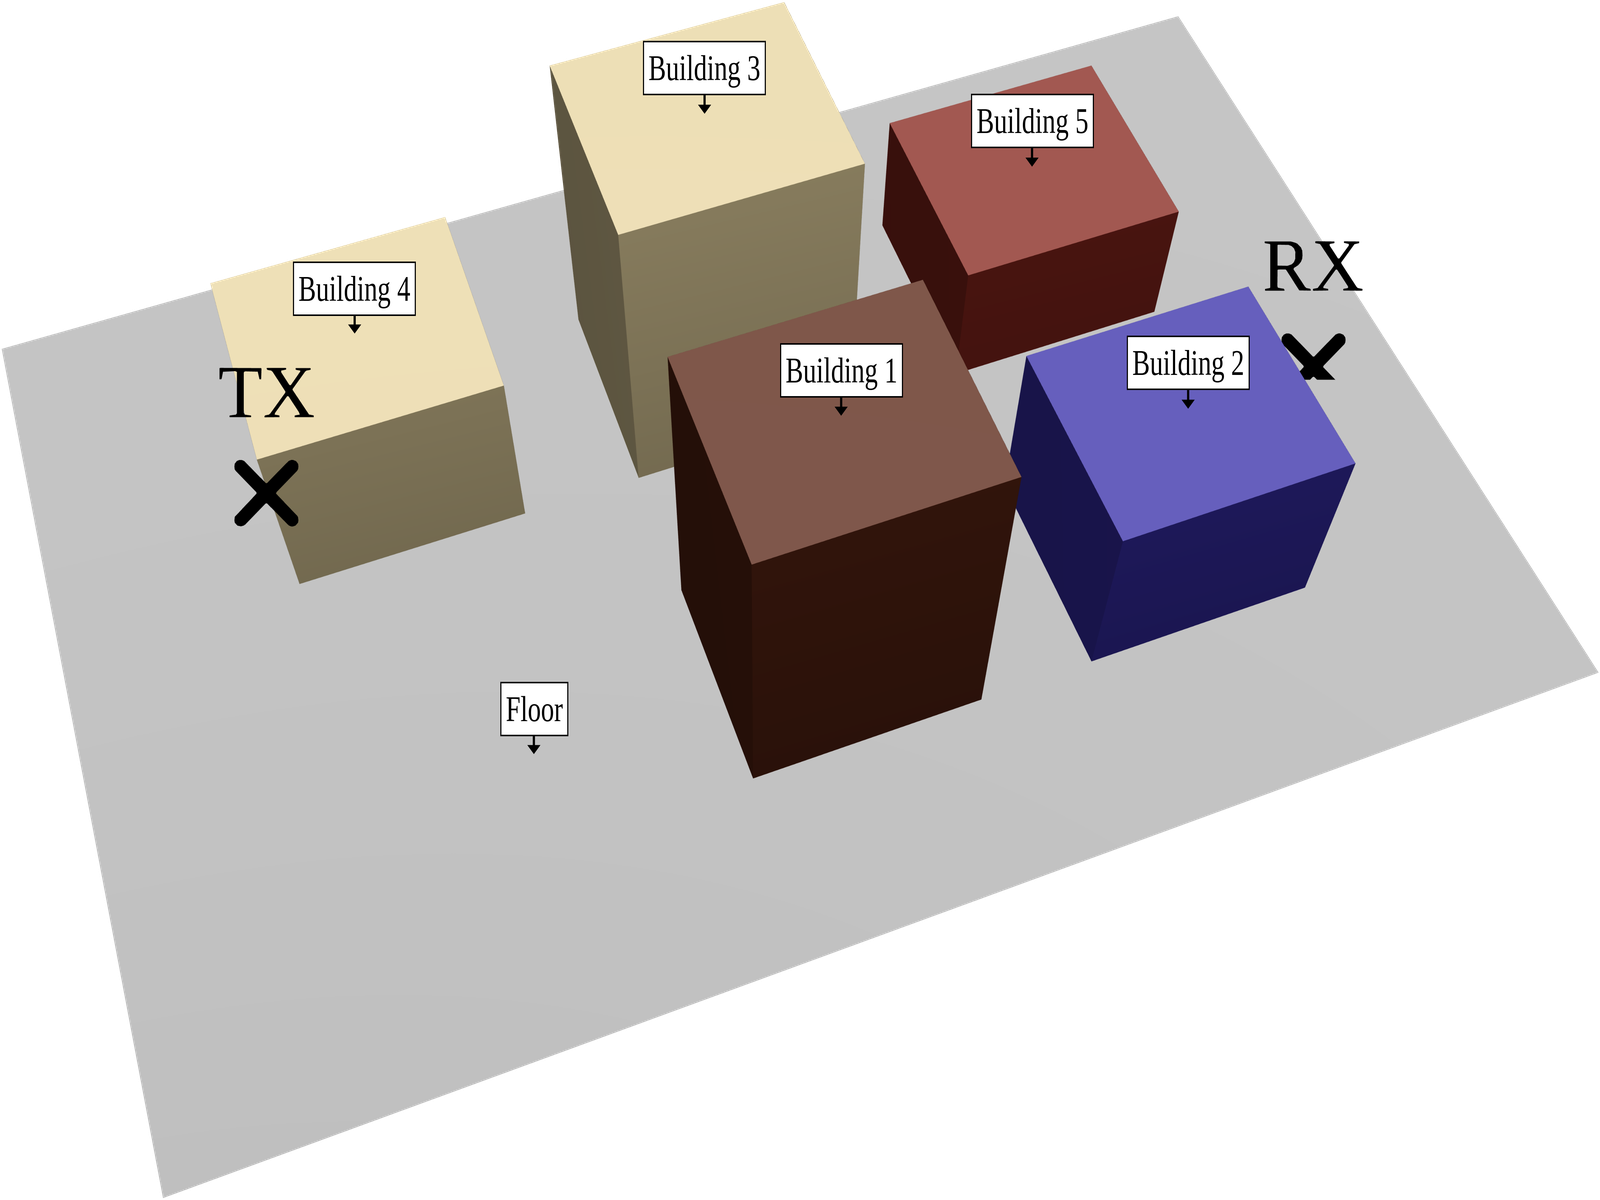
\includegraphics[width=\textwidth]{images/random-scene-annotated.png}
  \caption{3D idealized street canyon scene with annotated object identifiers used for the study of intermediate representations.}
  \labfig{research-gps-scene-plot}
\end{figure}

For each configuration, we extract three key internal outputs from the trained models of interaction orders $K \in \{1, 2, 3\}$: the object embeddings, the scene embeddings, and the step-by-step selection probability vectors.

\paragraph{Object Embeddings ($\bsit{Y}$)} The object encoder maps the canonical coordinates of the active triangles in the mesh to a 128-dimensional embedding space. The resulting embedding matrix $\bsit{Y}$ contains one row per triangle in the scene, where the $i$-th row stores the embedding vector $\bsit{y}_i$ of the corresponding triangle primitive. In other words, each horizontal strip in the matrix represents the learned features of a single object, while the columns correspond to the 128 embedding dimensions. In the canonical frame, the transmitter is always mapped to $
\begin{bmatrix}0 & 0 & 0
\end{bmatrix}^\top$ and the receiver to $
\begin{bmatrix}0 & 0 & 1
\end{bmatrix}^\top$. Swapping the transmitter and receiver shifts the origin and reverses the orientation of the reference axis, causing the canonical coordinates of all scene objects to change.

\reffig{research-gps-objects-embeddings} compares the resulting object embedding matrices for the basic and swapped scenes across orders 1, 2, and 3. The horizontal dashed lines indicate the boundaries between physical objects, with each object consisting of multiple triangles. These delimitations are only a visual aid: the model receives triangle-level geometry and is not given explicit information about which triangles belong to the same building. We observe that:
\begin{itemize}
  \item Triangles belonging to the same object exhibit highly coherent and uniform embedding values across the 128 dimensions. This indicates that the object encoder successfully aggregates local triangle geometries into object-level spatial features.
  \item Under the \glsxtrshort{tx}--\glsxtrshort{rx} swap, the activation patterns across the embedding dimensions change completely. This demonstrates that the encoder does not memorize invariant object identities; instead, it learns relative spatial representations tied to the canonical \glsxtrshort{tx}--\glsxtrshort{rx} propagation axis.
\end{itemize}

Furthermore, certain objects (such as Building 4 for the basic scene and Building 5 for the swapped scene, in the order $K=1$ embedding) exhibit faded, near-zero activations across the embedding dimensions. This occurs because these buildings do not lie on any geometrically valid first-order reflection paths between the transmitter and receiver. The object encoder learns to assign neutral, zero-valued feature vectors to these irrelevant components, effectively pruning them from downstream path selection. For $K=2$, a similar pattern can be observed for the same buildings. The higher the interaction order, the more objects can possibly lie on reflection paths, and hence the less pronounced this effect becomes.

\begin{figure*}
  \ContinuedFloat*
  \centering
  \begin{subfigure}[b]{\contentwidth}
    \centering
    \inputtikz{objects-embeddings-order1}
    \caption{Interaction order $K=1$ ($r = 0.0493$).}
    \labfig{research-gps-objects-embeddings-order1}
  \end{subfigure}

  \begin{subfigure}[b]{\contentwidth}
    \centering
    \inputtikz{objects-embeddings-order2}
    \caption{Interaction order $K=2$ ($r = 0.0250$).}
    \labfig{research-gps-objects-embeddings-order2}
  \end{subfigure}
  \caption{Comparison of intermediate object embeddings $\bsit{Y}$ for the basic scene (left) and the transmitter--receiver swapped scene (right) across interaction orders $K \in \{1, 2, 3\}$. The colorscale indicates the embedding values. The horizontal dashed lines demarcate boundaries between physical objects (buildings and floor). The distinct activation patterns demonstrate that the learned representations are coordinate-dependent. The Pearson correlation coefficient $r$ reported in each subfigure measures the correlation between the flattened object embedding matrices of the basic and swapped configurations.}
  \labfig{research-gps-objects-embeddings}
\end{figure*}

\begin{figure*}
  \ContinuedFloat
  \centering
  \begin{subfigure}[b]{\contentwidth}
    \centering
    \inputtikz{objects-embeddings-order3}
    \caption{Interaction order $K=3$ ($r = 0.0955$).}
    \labfig{research-gps-objects-embeddings-order3}
  \end{subfigure}
  \caption{Comparison of intermediate object embeddings $\bsit{Y}$ for the basic scene (left) and the transmitter--receiver swapped scene (right) across interaction orders $K \in \{1, 2, 3\}$ (continued). The colorscale indicates the embedding values. The horizontal dashed lines demarcate boundaries between physical objects (buildings and floor). The distinct activation patterns demonstrate that the learned representations are coordinate-dependent. The Pearson correlation coefficient $r$ reported in each subfigure measures the correlation between the flattened object embedding matrices of the basic and swapped configurations.}
\end{figure*}

\paragraph{Scene Embeddings} The scene encoder combines the individual object embeddings into a single 128-dimensional vector, representing the global scene state. \reffig{research-gps-scene-embeddings} stacks the scene embedding vectors for the basic and swapped configurations. Despite the coordinate transformation and the distinct patterns in individual object embeddings, certain dimensions of the scene representation remain partially correlated or stable under the swap. This indicates that the scene encoder preserves global spatial information (such as building density and spacing) while also capturing the orientation of the propagation axis.

To quantify the degree of symmetry preserved by the scene representation, we calculate the Pearson correlation coefficient $r$ between the embedding vector (or matrix) of the basic scene and that of the swapped scene. Specifically, for two flattened embeddings $\bsit{x}$ and $\bsit{y}$ of dimension $D$, the correlation coefficient is computed as
\begin{equation}
  r = \frac{\sum\limits_{i=1}^{D} (x_i - \bar{x})(y_i - \bar{y})}{\sqrt{\sum\limits_{i=1}^{D} (x_i - \bar{x})^2 \sum\limits_{i=1}^{D} (y_i - \bar{y})^2}},
\end{equation}
where $\bar{x} = \tfrac{1}{D}\sum_{i=1}^D x_i$ and $\bar{y} = \tfrac{1}{D}\sum_{i=1}^D y_i$ denote their respective sample means. Across the different interaction orders, we find a remarkably high correlation for the scene embeddings: $r = 0.9298$ for $K=1$, $r = 0.9278$ for $K=2$, and $r = 0.9321$ for $K=3$. This strong correlation ($\approx 0.93$) indicates that the combined scene representation is highly reciprocal and invariant to coordinate reflections. In comparison, the individual object embeddings $\bsit{Y}$ exhibit a very low correlation when flattened ($r = 0.0493$, $r = 0.0250$, and $r = 0.0955$ for $K=1, 2, 3$, respectively), highlighting that the object-level features remain coordinate-dependent while the pooled scene-level features achieve spatial reciprocity.

\begin{figure*}
  \centering
  \begin{subfigure}[b]{\contentwidth}
    \centering
    \inputtikz{scene-embeddings-order1}
    \caption{Interaction order $K=1$ ($r = 0.9298$).}
    \labfig{research-gps-scene-embeddings-order1}
  \end{subfigure}

  \begin{subfigure}[b]{\contentwidth}
    \centering
    \inputtikz{scene-embeddings-order2}
    \caption{Interaction order $K=2$ ($r = 0.9278$).}
    \labfig{research-gps-scene-embeddings-order2}
  \end{subfigure}

  \begin{subfigure}[b]{\contentwidth}
    \centering
    \inputtikz{scene-embeddings-order3}
    \caption{Interaction order $K=3$ ($r = 0.9321$).}
    \labfig{research-gps-scene-embeddings-order3}
  \end{subfigure}
  \caption{Comparison of scene embedding vectors for the basic scene (top row) and the transmitter--receiver swapped scene (bottom row) across interaction orders $K \in \{1, 2, 3\}$. The horizontal dashed line separates the two configurations. The Pearson correlation coefficient $r$ reported in each subfigure measures the correlation between the scene embedding vectors of the basic and swapped configurations. The high correlation ($\approx 0.93$) between the two configurations shows that global topological structures are preserved despite the coordinate reflection.}
  \labfig{research-gps-scene-embeddings}
\end{figure*}

\paragraph{Probability Vectors and Path Trajectories} The flow head generates selection policies (normalized edge flows) at each step of the path construction. \reffig{research-gps-probability-vectors} visualizes these step-by-step selection probabilities, with red boxes highlighting the selected objects at each interaction step.

The probability vectors show that the policy is highly sparse, concentrating almost all probability mass on a small subset of candidate objects, which confirms that the model successfully prunes unreachable or invalid parts of the search space.

Although the sampled path trajectories may differ (for example, at order $K=3$, the basic model samples $\text{Building } 4 \rightarrow \text{Building } 1 \rightarrow \text{Floor}$ while the swapped model samples $\text{Building } 5 \rightarrow \text{Building } 4 \rightarrow \text{Building } 4$), this difference is primarily a consequence of the stochastic sampling process during path candidate construction. Indeed, because sampling involves a random selection step, minor floating-point variations in the probability vectors can lead to different discrete path samples, even when using the same random seed. A closer examination of the selection probability vectors at the initial step (interaction index 0, before any object has been chosen) reveals a close match between the basic and swapped configurations across all orders. This indicates that the policy network has successfully learned reciprocal initial distributions. However, once a different first object is stochastically sampled, the subsequent probability distributions (at indices 1 and 2) naturally diverge because they are conditioned on different path histories. To fully align these conditional sequential policies and ensure reciprocal symmetry throughout the entire autoregressive generation process, symmetric training strategies, such as the transmitter--receiver symmetry replay described in \refsec{ml-assisted-rt}, remain crucial.

\begin{figure*}
  \centering
  \begin{subfigure}[b]{\contentwidth}
    \centering
    \inputtikz{probability-vectors-order1}
    \caption{Interaction order $K=1$ (one step).}
    \labfig{research-gps-probability-vectors-order1}
  \end{subfigure}

  \begin{subfigure}[b]{\contentwidth}
    \centering
    \inputtikz{probability-vectors-order2}
    \caption{Interaction order $K=2$ (two steps).}
    \labfig{research-gps-probability-vectors-order2}
  \end{subfigure}

  \begin{subfigure}[b]{\contentwidth}
    \centering
    \inputtikz{probability-vectors-order3}
    \caption{Interaction order $K=3$ (three steps).}
    \labfig{research-gps-probability-vectors-order3}
  \end{subfigure}
  \caption{Comparison of selection probability vectors (normalized edge flows) for the basic scene (left) and the transmitter--receiver swapped scene (right) across interaction orders $K \in \{1, 2, 3\}$. The colorscale indicates selection probability. Red boxes outline the selected object at each construction step, and vertical dashed lines denote boundaries between physical objects. The policy exhibits high sparsity, but trajectories differ due to the directional, random nature of path construction.}
  \labfig{research-gps-probability-vectors}
\end{figure*}

\subsection{Generalization to Unseen Scenarios and Sampling-Size Trade-Off}

\begin{figure*}
  \centering
  \inputtikz{ablation-sampling-size}
  \caption{Hit rate as a function of the number of samples $M$ for different training and evaluation sampling regions. The top row shows evaluation on the same sampling region as the training dataset, while the bottom row shows evaluation on a different sampling region (except for the whole scene case).}
  \labfig{ablation-sampling-size}
\end{figure*}

By design, the model is trained on randomized scenes to learn geometric properties rather than memorizing a single map. Although evaluation is performed on unseen snapshots, training and evaluation distributions can remain close when the transmitter and receiver are sampled from similar spatial regions. Complementing the journal results~\sidecite{Eertmans2026NPJWT}, \reffig{ablation-sampling-size} reports two additional analyses: (i) hit-rate evolution versus sampling budget $M$, and (ii) in-distribution versus shifted-distribution evaluation regions.

Most curves exhibit a saturation behavior: the hit rate increases quickly for small $M$ and then plateaus, typically around $M\approx 10$, consistent with the evaluation budget used in~\sidecite{Eertmans2026NPJWT}. This indicates diminishing returns from additional samples once dominant valid branches are already captured.

Evaluation on the same sampling region as training generally yields higher hit rates than evaluation on shifted regions, confirming a non-negligible distribution-shift effect. This gap is also visible in the coverage reconstructions of \reffig{predicted-coverage-maps}, with the exhaustive reference in \reffig{research-gps-gt}, the \gls{co} prediction in \reffig{research-gps-pred-co}, and the \gls{ws} prediction in \reffig{research-gps-pred-ws}. At the same time, models trained on broader spatial regions tend to degrade less under a distribution shift, indicating that training-region diversity improves robustness even when peak in-region performance is lower. Importantly, these coverage maps are defined using a \emph{non-coherent addition} of path powers, as introduced in \refsec{computing-total-channel}, to provide a stable estimate of the local mean power.

\begin{figure*}
  \centering
  \begin{subfigure}[t]{0.32\contentwidth}
    \centering
    \import{pgf/}{exhau.pgf}
    \caption{Ground truth (exhaustive).}
    \labfig{research-gps-gt}
  \end{subfigure}
  \hfill
  \begin{subfigure}[t]{0.32\contentwidth}
    \centering
    \import{pgf/}{pred-co.pgf}
    \caption{Prediction (trained on \gls{co}).}
    \labfig{research-gps-pred-co}
  \end{subfigure}
  \hfill
  \begin{subfigure}[t]{0.32\contentwidth}
    \centering
    \import{pgf/}{pred-ws.pgf}
    \caption{Prediction (trained on \gls{ws}).}
    \labfig{research-gps-pred-ws}
  \end{subfigure}
  \caption{Received power map reconstruction in log scale with the generative sampler (sampling size $M=10$) against the exhaustive ground-truth approach. The left plot shows the ground-truth coverage map obtained with exhaustive ray tracing, while the middle and right plots show the predicted coverage maps obtained with the generative sampler trained on the \gls{co} and \gls{ws} training scenarios, respectively.}
  \labfig{predicted-coverage-maps}
\end{figure*}

The root mean squared error between the predicted and exhaustive coverage maps in \reffig{predicted-coverage-maps} is \qty{3.48}{\decibel} (and \qty{1.62}{\decibel} when restricting evaluation to the canyon) for the \gls{co} model, and about \qty{2.41}{\decibel} (and \qty{1.36}{\decibel} when restricting evaluation to the canyon) for the \gls{ws} model. The stronger \gls{ws} performance, including inside the canyon, is consistent with better cross-region generalization.

To assess the generalization capability of the model on unseen urban environments with different structural properties, we evaluate the trained \gls{ws} model on real-world street-canyon scenarios obtained from OpenStreetMap data in Manhattan, New York. These scenarios exhibit structural characteristics distinct from the training distribution, including different building aspect ratios, facade complexity, street widths, and block organization patterns. Specifically, we select two test environments: a small scene with $N=400$ triangular facets and a medium scene with $N=805$ triangular facets, as shown in \reffig{research-manhattan-scenes}. Compared to the procedurally generated canyon training configurations (which contain up to $N=74$ facets), these real-world geometries represent a genuine out-of-distribution test case. Due to the increased scene complexity, specular reflections are evaluated up to second order ($K=2$), and the sampling budget is set to $M=100$ per receiver point to account for the higher density of potential propagation paths.

\begin{figure*}
  \centering
  \begin{subfigure}[t]{0.48\contentwidth}
    \centering
    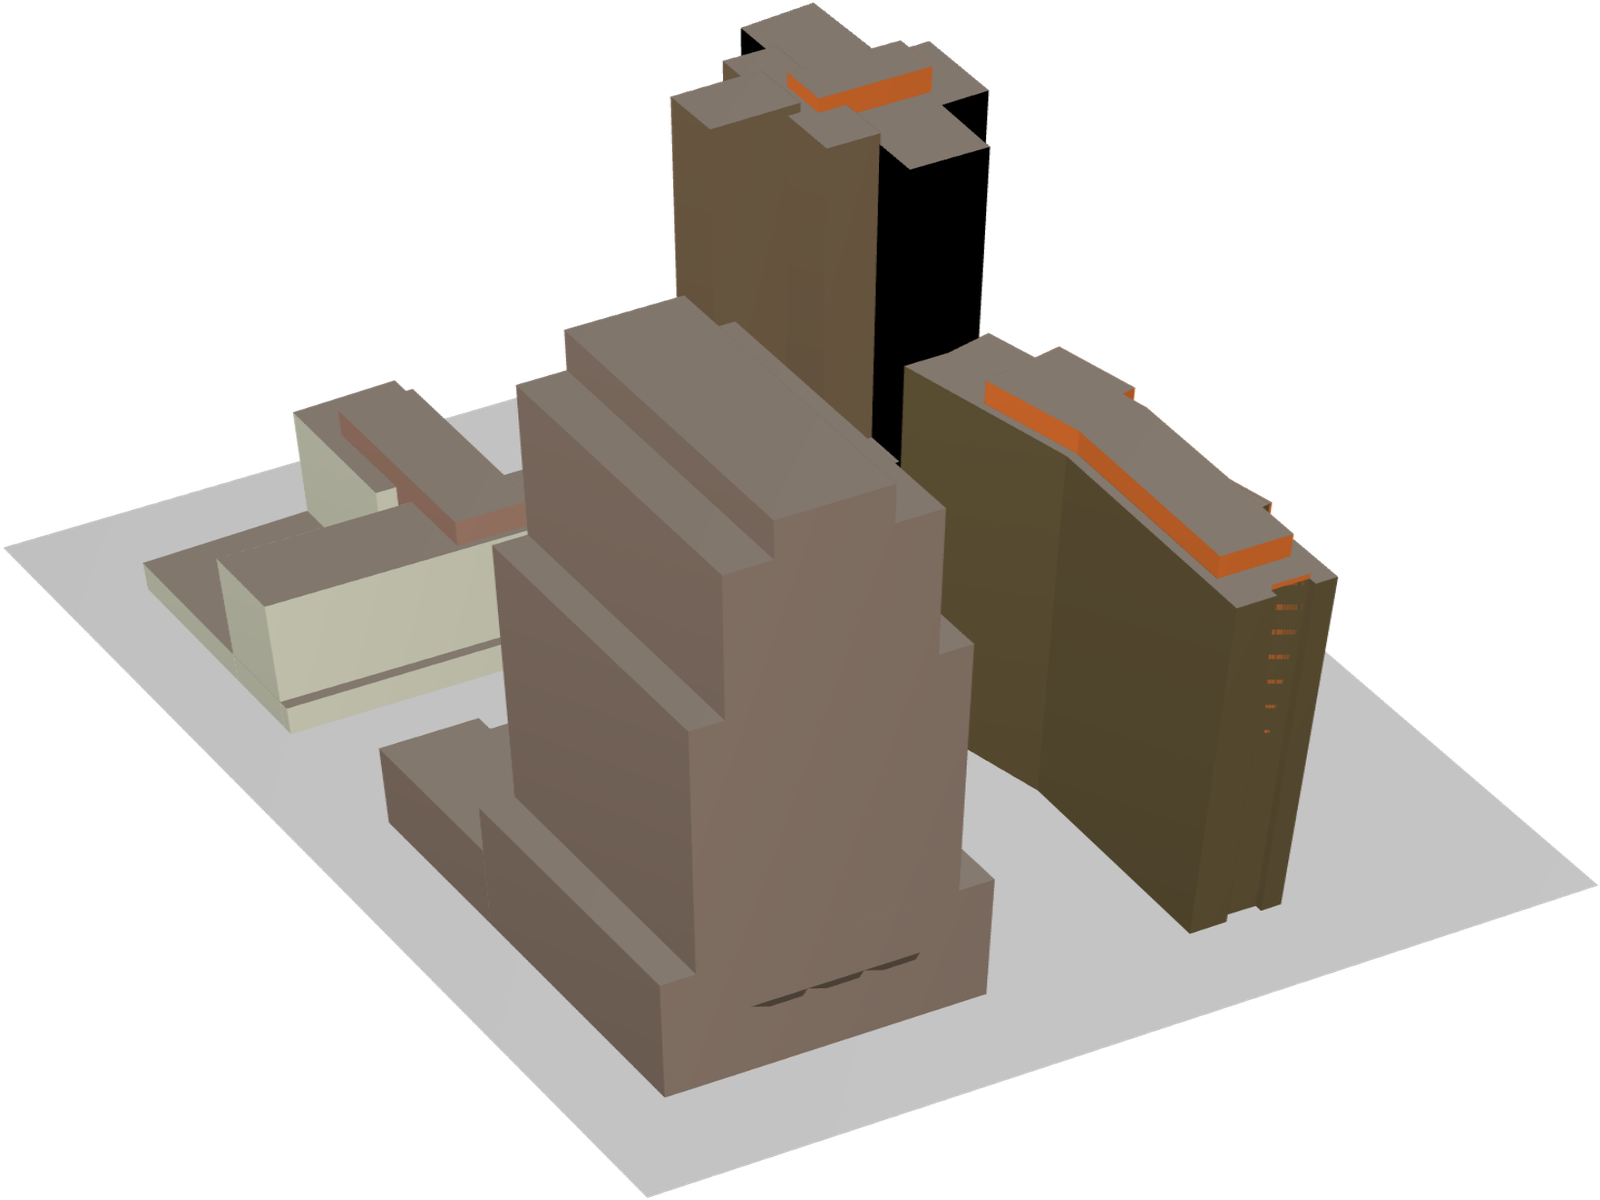
\includegraphics[width=\textwidth]{images/scene_400.png}
    \caption{Small scene ($N=400$ triangular facets).}
    \labfig{research-manhattan-small}
  \end{subfigure}
  \hfill
  \begin{subfigure}[t]{0.48\contentwidth}
    \centering
    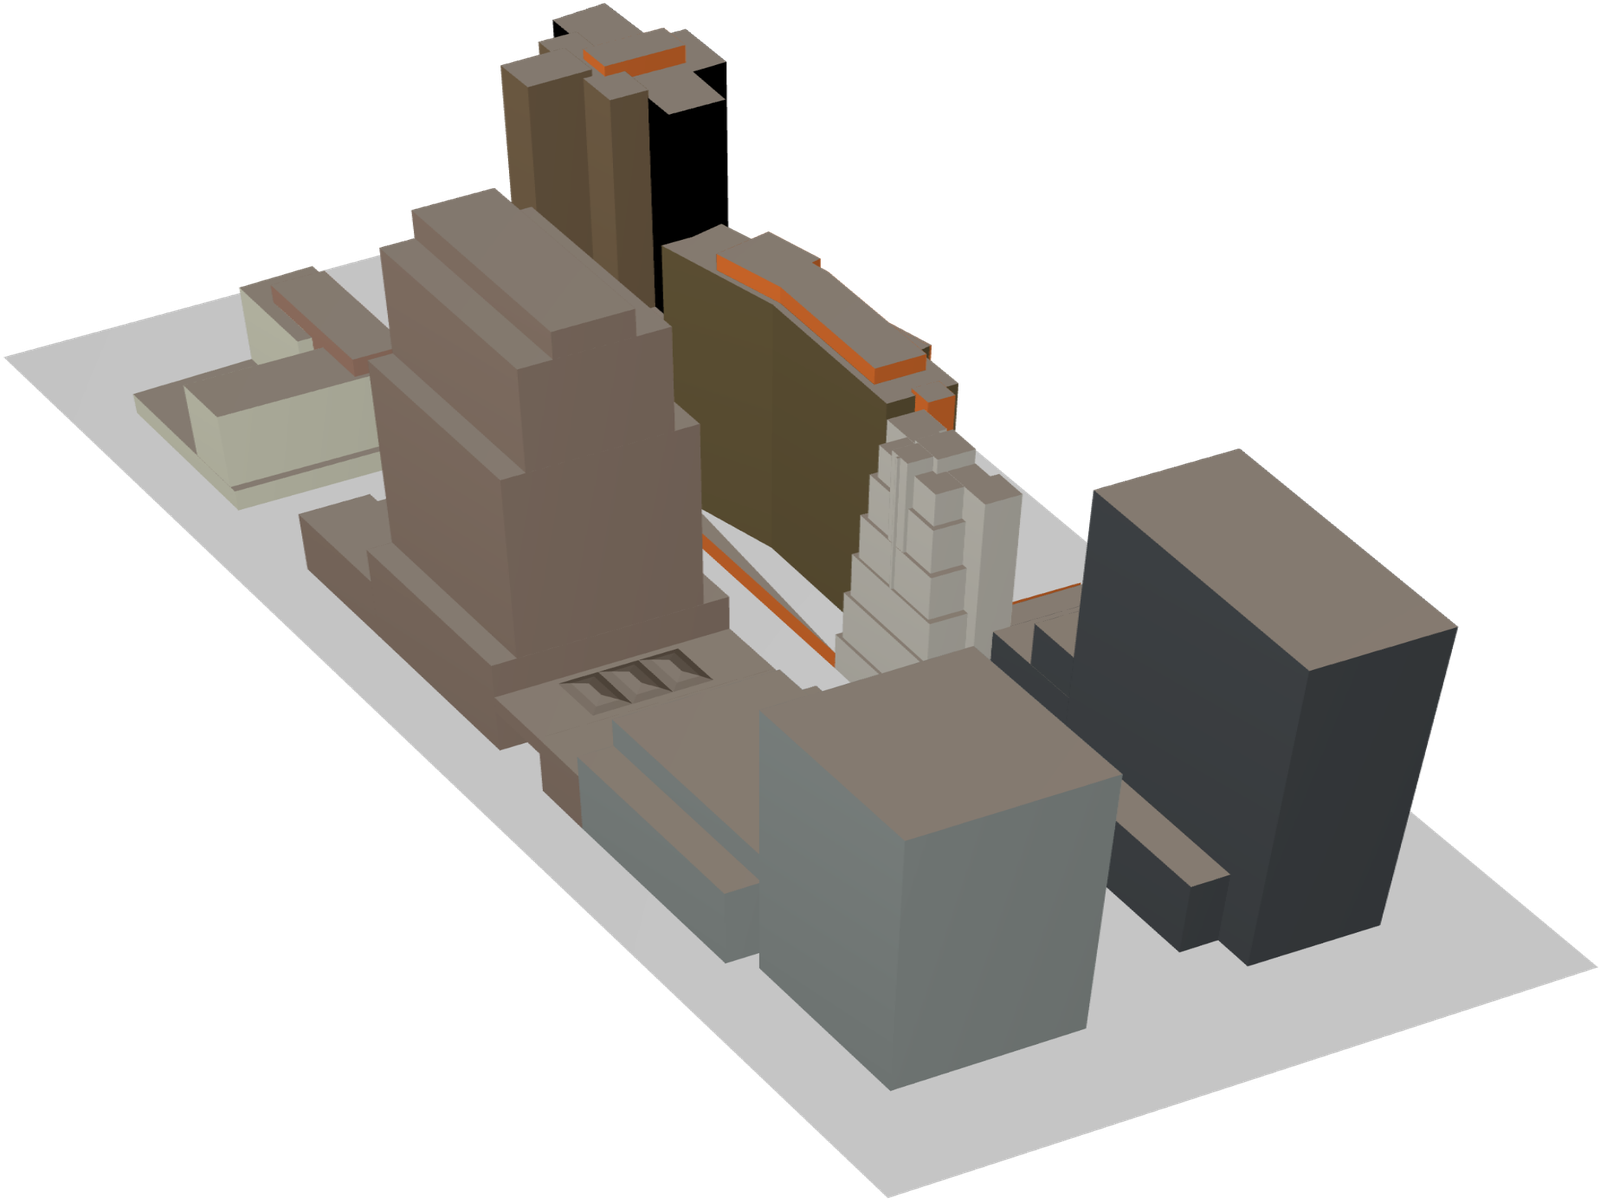
\includegraphics[width=\textwidth]{images/scene_805.png}
    \caption{Medium scene ($N=805$ triangular facets).}
    \labfig{research-manhattan-medium}
  \end{subfigure}
  \caption{Real-world Manhattan street canyon scenes obtained from OpenStreetMap. Both scenes exhibit different building aspect ratios, facade complexity, and street widths compared to the idealized training scenario.}
  \labfig{research-manhattan-scenes}
\end{figure*}

The resulting ground-truth and predicted coverage maps are compared in \reffig{research-manhattan-coverage-maps}. The evaluation highlights that while the model successfully discovers dominant reflection paths along the main street axes, its generalization to the out-of-distribution geometries is imperfect and exhibits significant spatial heterogeneity. The sampler reconstructs the general spatial distribution of the received power field reasonably well, but noticeable discrepancies from the ground truth emerge. Specifically, the prediction quality varies across different spatial regions: in some locations, the model fails to discover reflection paths from specific building facades, whereas in others, paths are only partially recovered. This spatial non-uniformity indicates that although the model has learned robust geometric regularities of path propagation that transfer beyond its procedural training configurations, it has not fully mastered general reflection principles and remains partially adapted to the structural regularities of the training family. Addressing this limitation to enable seamless transfer across arbitrary city layouts represents an important direction for future research, potentially through the use of increased model capacity, visibility-graph representations, or training on more complex scenarios from the outset.

\begin{figure*}[htbp]
  \centering
  \begin{subfigure}[t]{0.495\contentwidth}
    \centering
    \import{pgf/}{manhattan_small_exhau.pgf}
    \caption{Ground truth $G_{\mathrm{gt}}$ (small scene).}
    \labfig{research-manhattan-small-gt}
  \end{subfigure}
  \hfill
  \begin{subfigure}[t]{0.495\contentwidth}
    \centering
    \import{pgf/}{manhattan_small_pred.pgf}
    \caption{Prediction $G_{\mathrm{pred}}$ (small scene).}
    \labfig{research-manhattan-small-pred}
  \end{subfigure}
  \\
  \begin{subfigure}[t]{0.495\contentwidth}
    \centering
    \import{pgf/}{manhattan_medium_exhau.pgf}
    \caption{Ground truth $G_{\mathrm{gt}}$ (medium scene).}
    \labfig{research-manhattan-medium-gt}
  \end{subfigure}
  \hfill
  \begin{subfigure}[t]{0.495\contentwidth}
    \centering
    \import{pgf/}{manhattan_medium_pred.pgf}
    \caption{Prediction $G_{\mathrm{pred}}$ (medium scene).}
    \labfig{research-manhattan-medium-pred}
  \end{subfigure}
  \caption{Coverage map comparison for real, out-of-distribution Manhattan scenarios under a sampling budget of $M=100$, considering specular reflections up to second order. The plots compare the ground truth path gain (exhaustive) with the sampler's predictions for the small and medium scenes.}
  \labfig{research-manhattan-coverage-maps}
\end{figure*}

To assess the hardware robustness of the speed-up, the benchmark from~\sidecite{Eertmans2026NPJWT} is rerun on a different setup: 11\textsuperscript{th} Gen Intel\textcopyright{} Core\texttrademark{} i7-1165G7 $\times$ 8 (\gls{cpu}) and NVIDIA Quadro RTX\texttrademark{} 4000 (\gls{gpu}). Despite the hardware change, the acceleration trend remains consistent (\reffig{research-gps-benchmarks}), with large \gls{cpu} gains and smaller but still substantial \gls{gpu} gains. The lower relative gain on \gls{gpu} stems from the fact that the exhaustive baseline is already heavily parallelized and optimized for high-throughput ray--facet intersections, which partially masks the combinatorial overhead in the relatively small scenes tested. On the \gls{cpu}, where intersection tests are more sequential, the sampler's ability to prune the candidate space yields a more dramatic reduction in absolute runtime.

While these results were obtained on scenes with a limited number of buildings (e.g., 6 buildings in the street canyon), they demonstrate a proof of concept for replacing combinatorial candidate enumeration with learned generation. To scale this approach to city-scale environments with hundreds of buildings, the generative sampler would need to be combined with spatial acceleration structures such as \glspl{bvh} (see \refsec{acceleration-structures}). Commercial ray tracing tools often achieve their performance through such structures; however, our focus here is on addressing the fundamental combinatorial bottleneck that remains even with spatial pruning, especially at high interaction orders.

\begin{figure*}
  \centering
  \inputtikz{sampling-benchmarks}
  \caption{Runtime comparison of the generative path sampler against exhaustive ray tracing. The top and bottom rows show \gls{cpu} and \gls{gpu} times, respectively, as a function of scene complexity (number of objects) for interaction orders $K \in \{1, 2, 3\}$. Each subplot presents results for different sampling budgets $M$, demonstrating substantial speedups with the learned approach: approximately $100\times$ on \gls{cpu} and $10\times$ on \gls{gpu} at $M=10$.}
  \labfig{research-gps-benchmarks}
\end{figure*}

\subsection{Summary and Practical Implications}

Machine-learning-assisted path sampling occupies a practical middle ground between exhaustive physical solvers and purely data-driven surrogates. It preserves interpretability and physical validity while addressing the combinatorial bottleneck. The main trade-off is the offline training cost for each scene family. For repeated evaluations in the same class of environments (coverage sweeps, dense optimization loops, repeated \gls{tx} or \gls{rx} placements), the amortized runtime gain justifies this upfront investment. Together with the reconstruction errors reported above, these results support learned candidate generation as a robust acceleration layer for high-fidelity ray tracing.

\section{Study of the \texorpdfstring{\glsentrytitlecase{mlm}{long}}{Multipath Lifetime Map}}\labsec{mlm}

Where the previous section focused on computational efficiency through intelligent sampling, this section addresses a complementary question raised in \refch{efficient-path-tracing}: when and where can a ray tracing snapshot be safely extrapolated in dynamic scenarios? The \gls{mlm} is a geometric-topological construct that characterizes the validity of snapshot extrapolation in a chosen configuration-parameter space and provides quantitative measures to support hybrid workflows that combine local extrapolation with full recomputation only where necessary~\sidecite{Eertmans2025EuCAP}.

\subsection{Methodology}

As in the previous section, each ray path is described by a path candidate, i.e., an ordered list of interactions (interaction type and object identity). Let $\mathcal{I}^K$ be the set of all candidates up to interaction order $K$, and let $\mathcal{V}^K(\bsit{\theta})\subseteq\mathcal{I}^K$ be the subset that is geometrically valid for a given scene configuration $\bsit{\theta}$ (for example, receiver position, antenna tilt, or other dynamic scene parameters). Two scene configurations are treated as equivalent when they lead to the same valid-candidate set,
\begin{equation}
  \bsit{\theta}_a \sim \bsit{\theta}_b \iff \mathcal{V}^K(\bsit{\theta}_a)=\mathcal{V}^K(\bsit{\theta}_b).
\end{equation}

A \emph{multipath cell} $C_i$ is a connected region of the considered configuration space in which this valid-candidate set does not change. \Cref{fig:research-mlm-cells-los,fig:research-mlm-cells-up,fig:research-mlm-cells-down} show examples for individual interaction families, while \reffig{research-mlm-cells-all} (grouped in \reffig{research-mlm-cells}) shows the combined valid-path structure.

\begin{figure*}
  \centering
  \begin{subfigure}[t]{0.24\contentwidth}
    \centering
    \inputtikz{multipath-1}
    \caption{\Gls{line-of-sight} only.}
    \labfig{research-mlm-cells-los}
  \end{subfigure}
  \hfill
  \begin{subfigure}[t]{0.24\contentwidth}
    \centering
    \inputtikz{multipath-2}
    \caption{Upper-wall reflection.}
    \labfig{research-mlm-cells-up}
  \end{subfigure}
  \hfill
  \begin{subfigure}[t]{0.24\contentwidth}
    \centering
    \inputtikz{multipath-3}
    \caption{Lower-wall reflection.}
    \labfig{research-mlm-cells-down}
  \end{subfigure}
  \hfill
  \begin{subfigure}[t]{0.24\contentwidth}
    \centering
    \inputtikz{multipath-0}
    \caption{All interactions combined.}
    \labfig{research-mlm-cells-all}
  \end{subfigure}
  \caption{Illustration of multipath cells for individual interaction families and for the combined valid-path structure. Colors encode unique multipath identities, with up to 11 distinct cells in \protect\reffig{research-mlm-cells-all}.}
  \labfig{research-mlm-cells}
\end{figure*}

While \glspl{mlm} are not limited to exhaustive ray tracing and can also be used with \gls{sbr} methods, the worst-case number of candidates is still governed by exhaustive enumeration. For a scene with $N$ objects and fixed interaction order $K$, exhaustive tracing evaluates up to $M = N(N-1)^{K-1}$ candidates. Each cell can therefore be encoded by a binary vector $v_i \in \{0,1\}^{M}$, where each entry indicates whether a candidate in $\mathcal{I}^K$ is valid.

However, storing dense vectors for all cells is impractical because $M$ grows combinatorially. To reduce memory usage, the implementation processes candidates in chunks and compresses each cell encoding into a persistent hash-based identifier. This approach, similar to the one used to avoid double-counting in \gls{sbr}, preserves consistent coloring across snapshots without storing full-length dense vectors, provided that the candidate ordering is consistent across runs and hash collisions do not occur.

Each cell $C_i$ is characterized by two complementary metrics in the chosen configuration-parameter space. The \emph{cell measure} is $S_i = \mathrm{meas}(C_i)$ (which reduces to an area in 2D spatial settings), and the \emph{average minimal inter-cell distance} is $\overline{d_i}$, defined through the parameter-space distance-to-exit
\begin{equation}
  d_i(\bsit{\theta}) = \min_{\bsit{\theta}' \notin C_i} \mathrm{dist}(\bsit{\theta}, \bsit{\theta}'), \qquad \bsit{\theta} \in C_i,
\end{equation}
where $\overline{d_i}$ is the average of $d_i(\bsit{\theta})$ over $C_i$ in the considered parameter space. Importantly, the units of $S_i$ and $\overline{d_i}$ depend on the configuration variables used to build the \gls{mlm}: they are not intrinsically \unit{\meter\squared} and \unit{\meter}. For example, if the configuration variable is an antenna rotation angle, the corresponding distance-like quantity is angular and the associated units follow that choice. In mobility settings such as a moving receiver, the configuration space is spatial, so $S_i$ and $\overline{d_i}$ naturally take the units \unit{\meter\squared} and \unit{\meter}, and a practical local time-based validity horizon is approximated as $t_i \approx \overline{d_i}/v$.

With the exception of parameter values located at the intersection of multiple cells, adjacent cells differ by exactly one candidate in their encoding. This implies a Hamming distance of one between neighboring binary vectors. This structural property naturally leads to incremental path-update strategies at cell boundaries.

\subsection{Example \texorpdfstring{\glsentrytitlecase{mlm}{longpl}}{Multipath Lifetime Maps}}

To generate an \gls{mlm} for receiver mobility in a given scenario, we sweep the receiver across a spatial grid and compute the valid-candidate set at each location. Here, we evaluate a grid of $600\times 600$ receiver positions at a height of \qty{1.5}{\meter}, with the transmitter fixed at a height of \qty{32}{\meter}, in the street-canyon example. Because this example focuses on mobility induced by receiver-position variations, the resulting \glspl{mlm} and related metrics can be visualized directly in 2D spatial maps. \Cref{fig:research-mlm-0,fig:research-mlm-1,fig:research-mlm-2} report order-specific \glspl{mlm} for \gls{line-of-sight}, first-order reflections, and second-order reflections, respectively.

These \glspl{mlm} differ from those reported in~\sidecite{Eertmans2025EuCAP}, where the analysis was performed for the combined \gls{line-of-sight} and first-order set. The order-separated views shown here provide finer structural insight: \gls{line-of-sight} \glspl{mlm} form broad and relatively simple regions, first-order \glspl{mlm} exhibit stronger fragmentation driven by reflection-visibility boundaries, and second-order \glspl{mlm} show the highest spatial complexity due to compounded interaction constraints.

\begin{figure*}
  \centering
  \begin{subfigure}[t]{0.49\contentwidth}
    \centering
    \import{pgf}{mlm-0-a.pgf}
    \caption{Initial \gls{tx} position.}
    \labfig{research-mlm-0-a}
  \end{subfigure}
  \begin{subfigure}[t]{0.49\contentwidth}
    \centering
    \import{pgf}{mlm-0-b.pgf}
    \caption{Intermediate \gls{tx} position.}
    \labfig{research-mlm-0-b}
  \end{subfigure}
  \caption{Example \glspl{mlm} across transmitter positions for \gls{line-of-sight} paths. Identical colors indicate identical multipath-cell identities across transmitter positions.}
  \labfig{research-mlm-0}
\end{figure*}

\begin{figure*}
  \centering
  \begin{subfigure}[t]{0.49\contentwidth}
    \centering
    \import{pgf}{mlm-1-a.pgf}
    \caption{Initial \gls{tx} position.}
    \labfig{research-mlm-1-a}
  \end{subfigure}
  \begin{subfigure}[t]{0.49\contentwidth}
    \centering
    \import{pgf}{mlm-1-b.pgf}
    \caption{Intermediate \gls{tx} position.}
    \labfig{research-mlm-1-b}
  \end{subfigure}
  \caption{Example \glspl{mlm} across transmitter positions for first-order reflection paths. Identical colors indicate identical multipath-cell identities across transmitter positions.}
  \labfig{research-mlm-1}
\end{figure*}

\begin{figure*}
  \centering
  \begin{subfigure}[t]{0.49\contentwidth}
    \centering
    \import{pgf}{mlm-2-a.pgf}
    \caption{Initial \gls{tx} position.}
    \labfig{research-mlm-2-a}
  \end{subfigure}
  \begin{subfigure}[t]{0.49\contentwidth}
    \centering
    \import{pgf}{mlm-2-b.pgf}
    \caption{Intermediate \gls{tx} position.}
    \labfig{research-mlm-2-b}
  \end{subfigure}
  \caption{Example \glspl{mlm} across transmitter positions for second-order reflection paths. Identical colors indicate identical multipath-cell identities across transmitter positions.}
  \labfig{research-mlm-2}
\end{figure*}

Quantitative statistics of the proposed metrics (cell-area distributions and average minimal inter-cell distances) are reported in~\sidecite{Eertmans2025EuCAP}.

\subsection{Practical Guidance and Extensions}

The \gls{mlm} reframes extrapolation validity as a geometric question measurable directly from path topology. This yields practical guidance: if trajectories remain within large cells, dynamic ray tracing via snapshot extrapolation is efficient; if trajectories cross many cell boundaries, full recomputation may become preferable.

Beyond receiver mobility, the methodology extends to other dynamic variables (moving reflectors, reconfigurable elements, and beam-state changes) and supports adaptive simulation strategies that balance fidelity and runtime. This perspective naturally connects to the chapter conclusion, which synthesizes both contributions.

\section{Conclusion}

This chapter has explored two complementary research directions that extend ray tracing beyond its classical deterministic formulation. First, the machine-learning-assisted path sampler shows how neural networks can complement physics-based simulation: instead of learning electromagnetic fields directly, the model identifies promising partial paths and delegates physical evaluation to geometric and electromagnetic solvers. The reported speedups---approximately $100\times$ on \gls{cpu} and $10\times$ on \gls{gpu} at evaluation budgets of $M=10$ samples---make high-fidelity multipath analysis tractable even in demanding scenarios. This efficiency, however, requires offline training for each scene family and is therefore most beneficial when many evaluations are amortized over the same environment class.

Second, the \gls{mlm} emphasizes reliability and validity. By characterizing where path topology remains stable, the \gls{mlm} enables hybrid workflows that combine fast extrapolation with full recomputation only at critical boundaries. This geometry-driven perspective aligns with physical intuition and provides actionable guidance for motion planning and simulation scheduling.

Together, these studies support a broader principle for computational propagation: machine learning and geometric analysis are most effective when they augment---rather than replace---fundamental physics. This chapter therefore closes the technical development of this book by establishing both an acceleration paradigm (learned path generation) and a validity paradigm (topology-aware extrapolation). Future work could further refine the generative sampler by integrating electromagnetic material properties (such as complex permittivity) into the object features, allowing the model to selectively prune interactions with highly lossy or diffuse surfaces.

In the next and final chapter, we will conclude on what we have seen and discuss the potential implications for future research and applications in differentiable ray tracing.
